
\documentclass[10pt]{beamer}

\usepackage[utf8]{inputenc}
\usepackage[T2A]{fontenc}
\usepackage[russian]{babel}
\usepackage{hyperref}
\usepackage{amsmath}
%\usepackage[footnotes,oglav,spisok,boldsect,eqwhole,kursrab,hyperprint]{project1}
\usetheme{Copenhagen}
\useoutertheme{default}
\usecolortheme{sidebartab}
%\usefonttheme{serif}
\useoutertheme[]{miniframes}
\usepackage{graphicx}
\usepackage{lipsum}
%\usepackage{rumathgrk1}
%\usepackage{glonti}
\defbeamertemplate*{footline}{Warsaw} {%
\leavevmode%
\hbox{%
\begin{beamercolorbox}[wd=.5\paperwidth,ht=2.5ex,dp=1.125ex,leftskip=.3cm,rightskip=.3cm]{author in head/foot}%
\insertframenumber{}%
\hfill\insertshortauthor
\end{beamercolorbox}%
\begin{beamercolorbox}[wd=.5\paperwidth,ht=2.5ex,dp=1.125ex,leftskip=.3cm,rightskip=.3cm]{title in head/foot}%
\usebeamerfont{title in head/foot}\insertshorttitle
\end{beamercolorbox}
}%
\vskip0pt%
}
% \setbeamersize
% {
%     text margin left=0.8cm,
%     text margin right=0.8cm
% }
\title{\textbf{Восстановление человеком исходной позы после толчка \\
Reversion of initial posture by a person after a push}}

\author{\textbf{Романов Андрей Владимирович}}
\institute{\textbf{МГУ им. М.В. Ломоносова}\\\textbf{Механико-математический факультет} 
\\ \textbf{Кафедра прикладной механики и управления}
\\ \textbf{Научный руководитель: Кручинин П.А.}}
\date{\today}



\begin{document}

\maketitle

\begin{frame}{Описание задачи}
	\begin{figure}[h!]
		\begin{center}
			\begin{minipage}[h]{0.33\linewidth}
				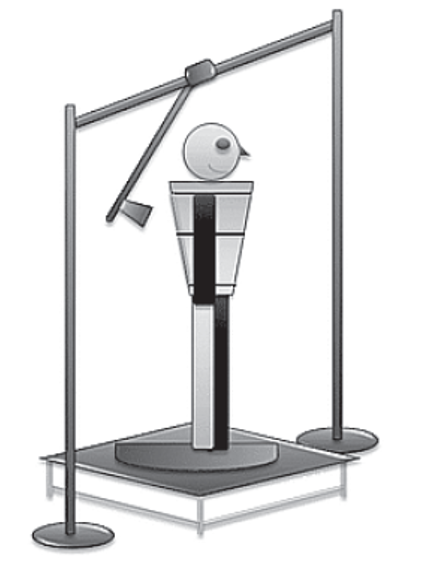
\includegraphics[width=1\linewidth]{images/human.png}
				\caption{Схематическое изображение толкателя
					и положения испытуемого на стабилоплатформе}
			\end{minipage}
			\hfill
			\begin{minipage}[h]{0.66\linewidth}
				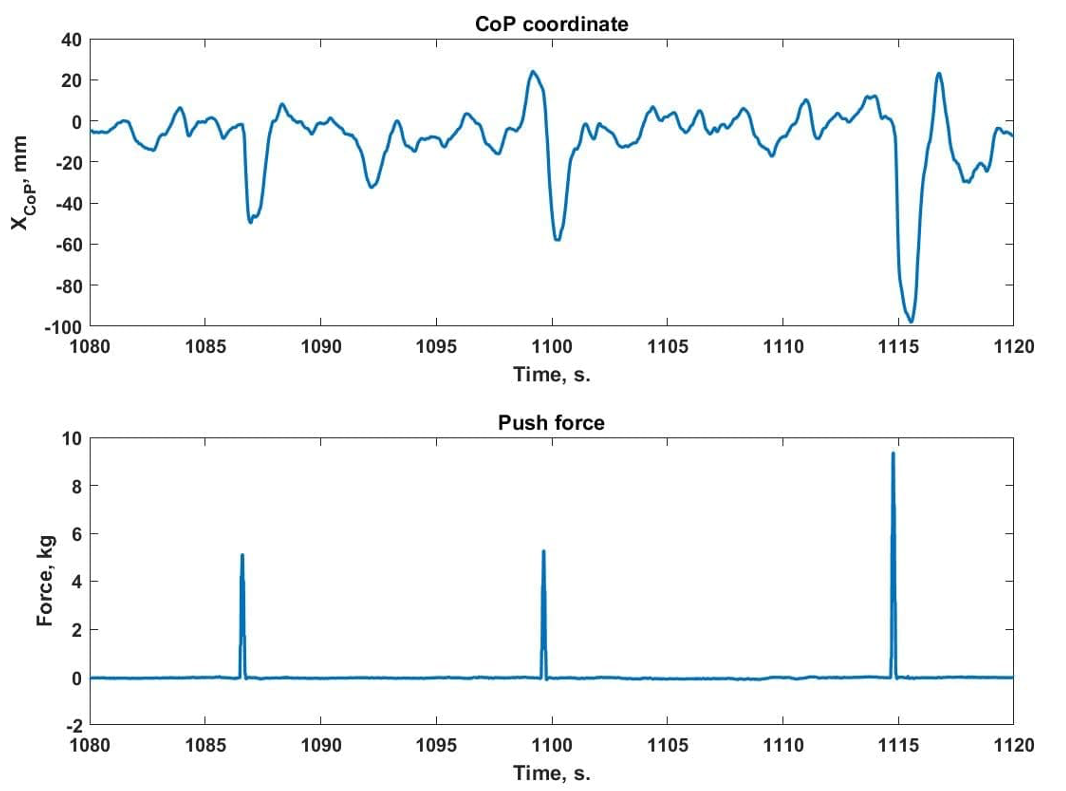
\includegraphics[width=1\linewidth]{images/Pushes.png}
				{\footnotesize
					\caption{Отклонение сагиттальной координаты при различных по силе толчках (данные предоставлены сотрудниками ИМБП РАН) }
				}
			\end{minipage}
		\end{center}
	\end{figure}
\end{frame}

\begin{frame}{Задача быстродействия}
	\begin{columns}
		\column{0.55\textwidth}
		\begin{figure}[h!]
			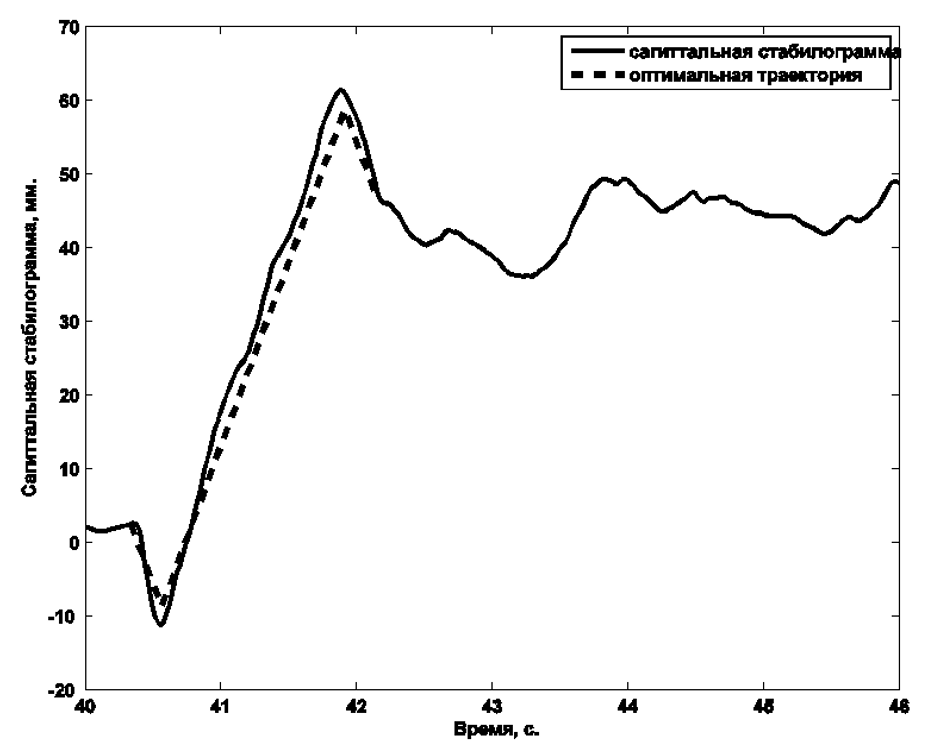
\includegraphics[width=1\linewidth]{images/stabilos.png}
			\caption{Характерный вид сагиттальной стабилограммы при выполнении теста со ступенчатым воздействием}
		\end{figure}
		\column{0.6\textwidth}
		% \column{\dimexpr\paperwidth-2pt}
		В работе рассматриваются возможные алгоритмы управления изменением
		позы человека, основанные на решении задачи оптимального быстродействия,
		которые можно было бы использовать для возвращения человека в исходную 
		вертикальную позу. В качестве математической модели используется модель
		«перевернутого маятника». Это решение предлагается использовать для
		оценки эффективности управления человеком при возвращении в
		вертикальную позу, путем сравнения времени реального процесса с полученным
		эталонным решением оптимальной задачи.
	\end{columns}
\end{frame}

\begin{frame}{Математическая модель}
	\begin{columns}
		\column{0.62\textwidth}
		\begin{figure}[h!]
			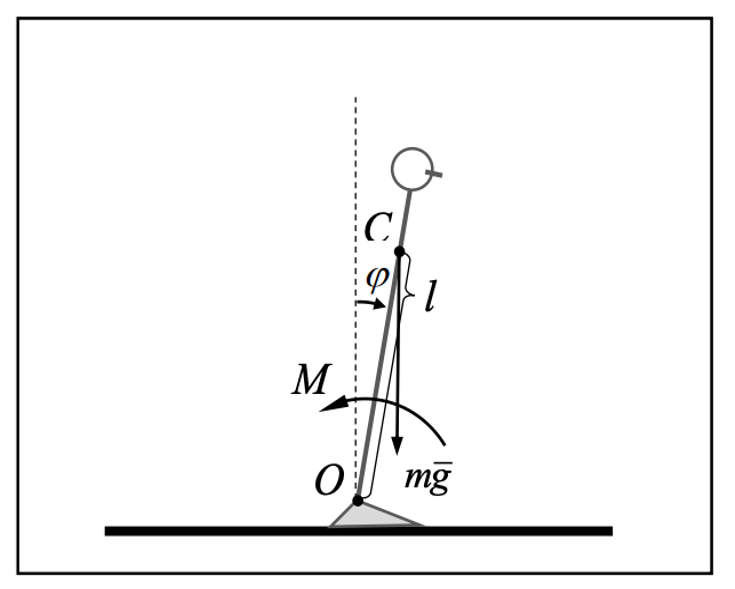
\includegraphics[width=1\linewidth]{images/inverse_pendulum.png}
			\caption{Модель перевернутого маятника}
		\end{figure}
		\column{0.5\textwidth}

		\[
			J\ddot{\varphi}=m_Tgl\varphi+M
		\]
		\[
			\varphi(0)=\varphi_0,\, \dot{\varphi}(0)=\omega_0
		\]
		\[
			\varphi(t)=\varphi_k,\, \dot{\varphi}(t_k)=0
		\]
		\[
			M(0)=M(t_k)=-m_Tgl\varphi_k
		\]
		\[
			U^-\leq\dot{M}\leq U^+
		\]
	\end{columns}
\end{frame}
\begin{frame}{Решение задачи быстродействия}
	В прошлом году решалась задача быстродействия

	Система разбивается на 3 этапа, на каждом из которых управление меняет знак

	В результате получилось численно-аналитическое решение, которое сводится к отысканию корней полинома для нахождения времени возвращения в вертикальную позицию.
	\begin{columns}
		\column{0.5\textwidth}
		\begin{equation}\label{koshisystem}
			\left\{ {\begin{aligned}
						 & \theta^{'} = \omega , \hfill   \\
						 & \omega^{'} = \theta+m , \hfill \\
						 & m^{'} = u . \hfill             \\
					\end{aligned}} \right.
		\end{equation}
		\column{0.5\textwidth}
		\[
			u=
			\begin{cases}
				-u_{max} \\
				+u_{max}
			\end{cases}
		\]\\*
	\end{columns}

\end{frame}

\begin{frame}{Связь центра масс и центра дваления}
		\begin{columns}
		\column{0.5\textwidth}
		\begin{figure}[h!]
			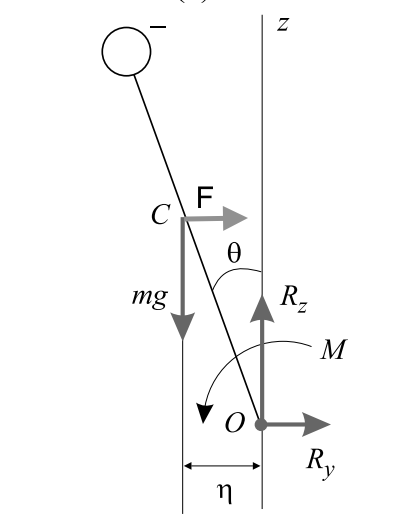
\includegraphics[width=0.8\linewidth]{images/body.png}
			\caption{Силы действующие на модель стержня, имитирующего тело человека}
		\end{figure}
		\column{0.5\textwidth}
		\begin{figure}[h!]
			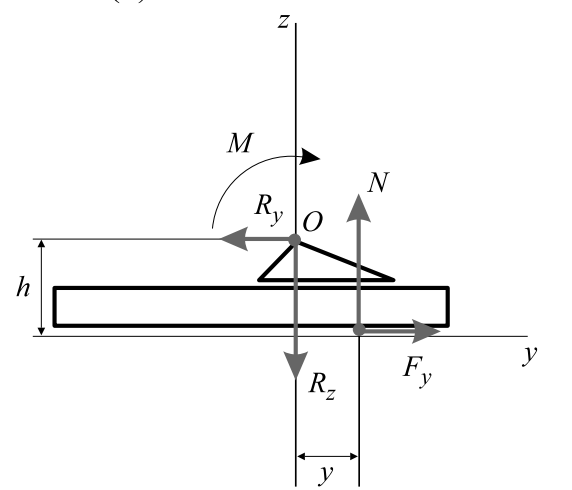
\includegraphics[width=0.8\linewidth]{images/foot.png}
			\caption{Силы действующие на на систему «стопы ног – платформа стабилоанализатора» }
		\end{figure}
	\end{columns}

\end{frame}

\begin{frame}{Связь центра масс и центра давления}
	\begin{columns}
	\column{0.5\textwidth}
	\begin{equation}\label{koshisystem}
    \left\{ {\begin{aligned}
                 & ml\ddot{\theta} = -R_y-F , \hfill   \\
                 & 0=R_z-mg, \hfill \\
                 & J \ddot{\theta} = mlg\theta-Fl+M_x . \hfill             \\
            \end{aligned}} \right.
\end{equation}
	\column{0.5\textwidth}
	\begin{equation}\label{koshisystem}
		\left\{ {\begin{aligned}
					 & M_x = Ny+F_yh , \hfill   \\
					 & F_y = R_y , \hfill \\
					 & N \approx mg . \hfill             \\
				\end{aligned}} \right.
	\end{equation}
\end{columns}

	$$M_x=mgy-h\left(F+ml\ddot{\theta}\right)$$

	$$\left(J+mlh\right)\ddot{\theta}=mgl\theta+mgy-Fl-Fh$$ 


 	$$\frac{(J+mlh)l\ddot{\theta}}{mgl}=l\theta+y-\frac{F}{mg}(l+h);\quad \text{Замена: }\eta=-l\theta; \quad T^2=\frac{J+mlh}{mgl};$$
\begin{equation}\label{eta_y}
	T^2\ddot{\eta}=\eta-y+\frac{F}{mg}(l+h)
\end{equation}

\end{frame}

\begin{frame}{Связь центра масс и центра давления}
	Cоотношение \eqref{eta_y} предлагается использовать для определения начальных условий движения сразу после толчка

	Дальнейший анализ сводится к задаче Коши
	\begin{equation}\label{eta_y_easy}
		T^2\ddot{\eta}=\eta-y
	\end{equation}
	C начальными условиями $\eta(0)=\eta_0; \dot{\eta}(0)=\nu_0$, найденными из \eqref{eta_y}.

	Далее необходимо построить оценку $\tilde\eta$ движения центра масс различными способами
\end{frame}

\begin{frame}{Моделирование движения человека}
	\begin{figure}[h!]
		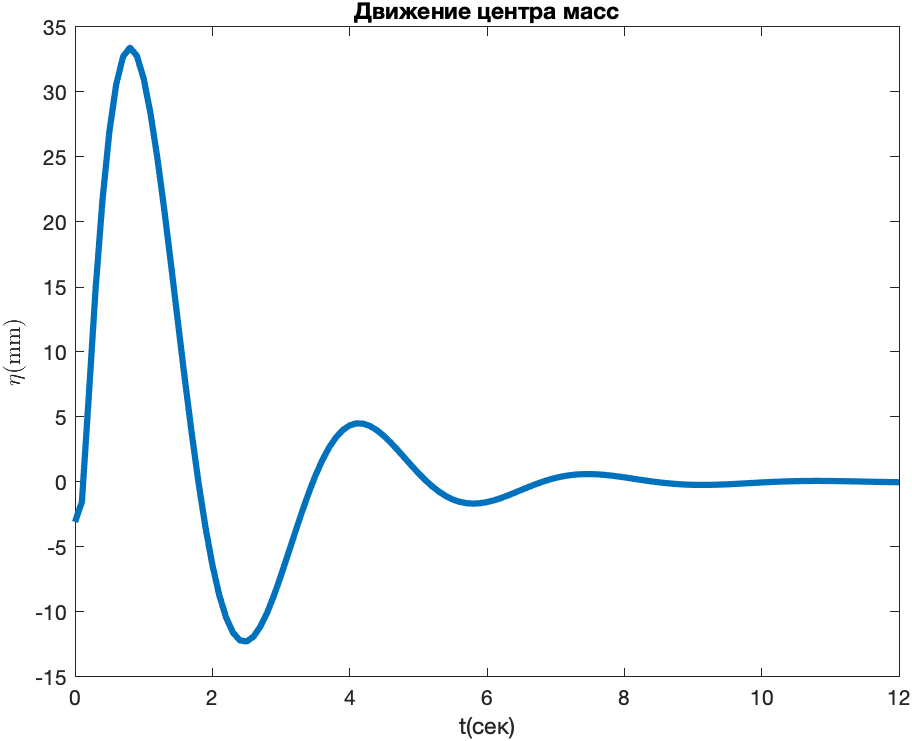
\includegraphics[width=0.7\linewidth]{images/center_mass_my.png}
		\caption{Модель изменения саггитальной координаты центра масс}
	\end{figure}
\end{frame}
\begin{frame}{Моделирование движения человека}
	\begin{columns}
		\column{0.5\textwidth}
		\begin{figure}[h!]
			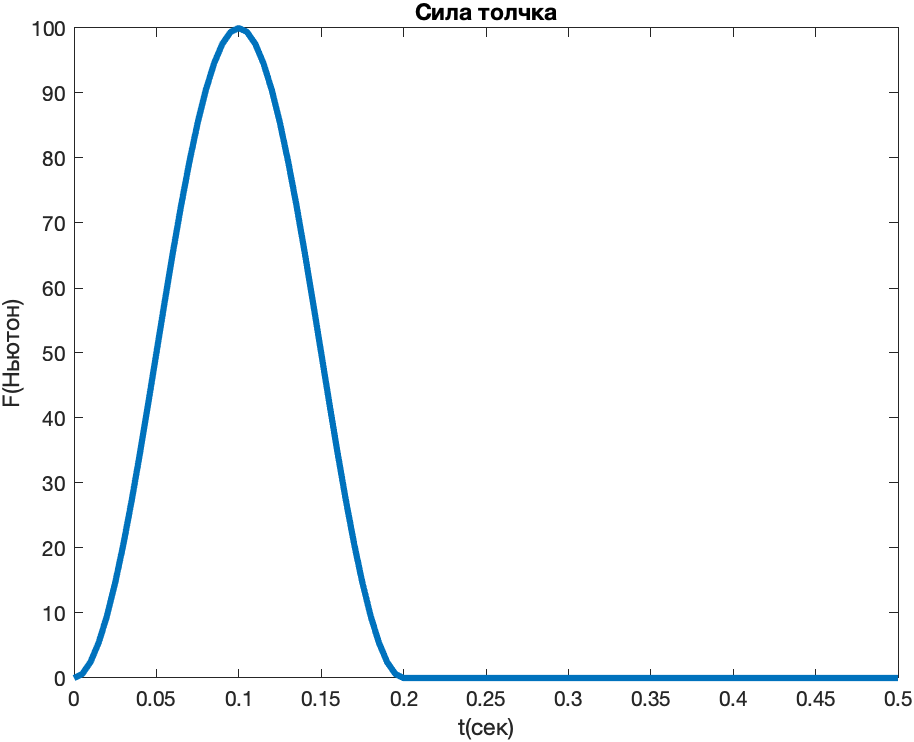
\includegraphics[width=1\linewidth]{images/pushes_my.png}
			\caption{Модель силы толчка}
		\end{figure}
		\column{0.6\textwidth}
		\begin{figure}[h!]
			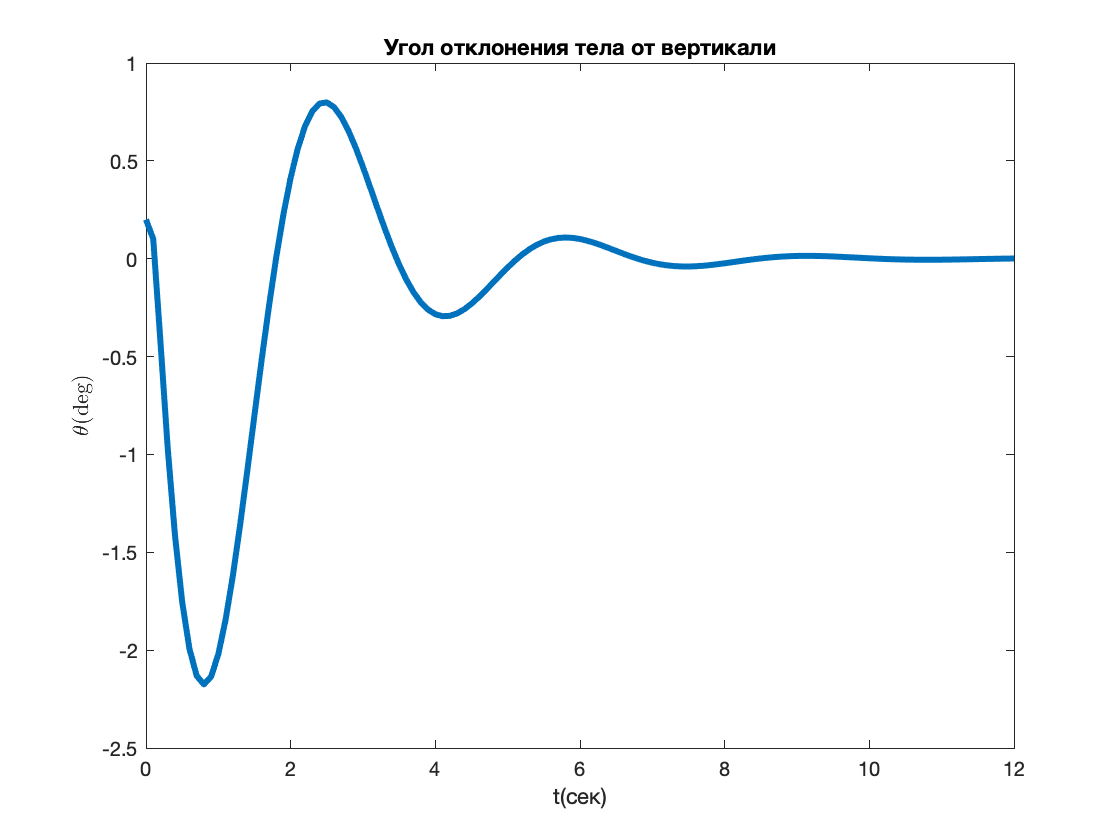
\includegraphics[width=1\linewidth]{images/degrees.png}
			\caption{Модель изменения угла отклонения}
		\end{figure}
	\end{columns}
\end{frame}
\begin{frame}{Моделирование движения человека}
	\begin{figure}[h!]
		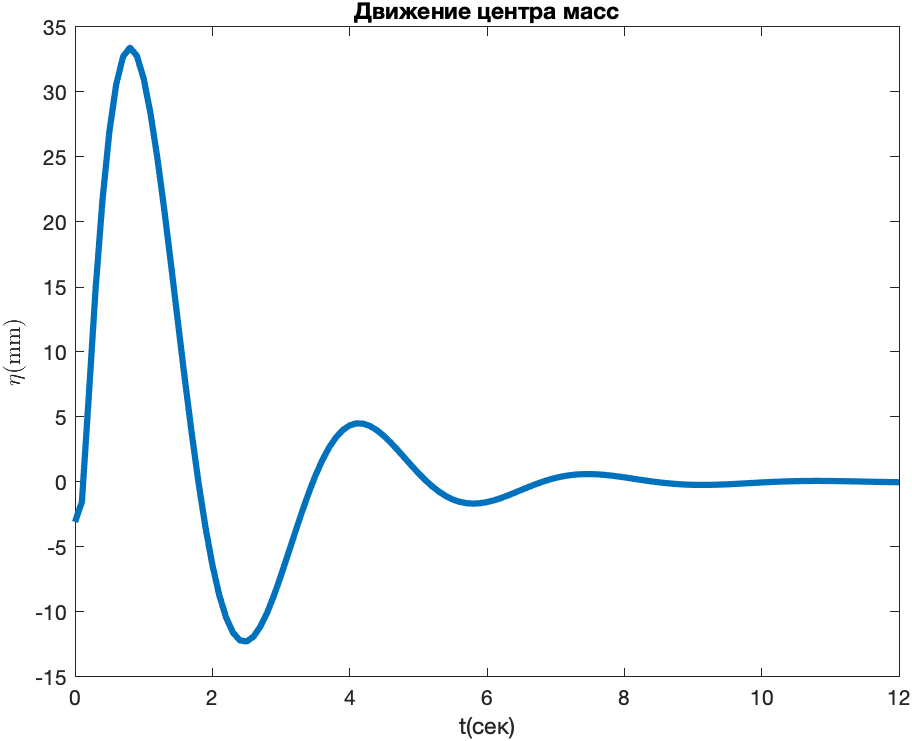
\includegraphics[width=0.7\linewidth]{images/center_mass_my.png}
		\caption{Модель изменения саггитальной координаты центра масс}
	\end{figure}
\end{frame}

\begin{frame}{Дальнейшие шаги}
	\begin{itemize}
		\item Провести дальнейшее моделирование и построить оценку траектории центра масс
		\item Сравнить реальное время возвращения в вертикальную позу с полученными при решении задачи быстродействия
		\item Построить траекторию центра масс при управленнии, полученном при решении задачи быстродействия
	  \end{itemize}
	
\end{frame}

\end{document}